% Shared vector grammar. Generated figure TeX files inline this source.
\documentclass[tikz,border=4mm,12pt]{standalone}
\usepackage[UTF8,fontset=fandol]{ctex}
\usepackage{amsmath,amssymb,bm}
\renewcommand{\familydefault}{\sfdefault}
\hyphenpenalty=10000
\exhyphenpenalty=10000
\usetikzlibrary{arrows.meta,backgrounds,calc}
\definecolor{Ink}{HTML}{273648}
\definecolor{Muted}{HTML}{607086}
\definecolor{Ctx}{HTML}{85898F}
\definecolor{Qst}{HTML}{4F8FA5}
\definecolor{Opt}{HTML}{5A9A6E}
\definecolor{Gen}{HTML}{B89A5E}
\definecolor{Hid}{HTML}{8A74B5}
\definecolor{Wgt}{HTML}{E0904F}
\definecolor{Lgt}{HTML}{C95B5B}
\definecolor{Idx}{HTML}{7E8B9B}
\definecolor{Msk}{HTML}{3F5A78}
\newcommand{\Unit}{0.30}
\newcommand{\Offset}{0.12}
\newcommand{\BinarySupport}{0}
\newcounter{texture}
\tikzset{
 flow/.style={-{Latex[length=2mm,width=1.5mm]},draw=Ink!75,line width=.65pt},
 tensorlabel/.style={font=\small,text=Ink,align=center,inner sep=0pt},
 tenshape/.style={font=\scriptsize,text=Muted,align=center,inner sep=0pt},
 stage/.style={font=\small\bfseries,text=Muted,align=left,anchor=west},
 operation/.style={draw=Ink!25,fill=white,rounded corners=2pt,align=center,
  font=\small,text=Ink,inner sep=5pt,line width=.5pt},
}
% The last two axes define a matrix face. Leading axes use offset sheets.
% Every symbolic dimension maps to the same cell count throughout the set.
\newcommand{\Tensor}[9]{%
 \stepcounter{texture}
 \pgfmathsetmacro{\ww}{#5*\Unit}
 \pgfmathsetmacro{\hh}{#4*\Unit}
 \pgfmathsetmacro{\xx}{#2-\ww/2}
 \pgfmathsetmacro{\yy}{#3-\hh/2}
 \ifnum#7>0
  \foreach \s in {#7,...,1}{
   \path[draw=#6!40,fill=white,line width=.45pt,rounded corners=.7pt]
    ({\xx+\s*\Offset},{\yy+\s*\Offset}) rectangle ++(\ww,\hh);}
 \fi
 \foreach \r in {1,...,#4}{\foreach \c in {1,...,#5}{
  \ifnum\BinarySupport>0
   \pgfmathtruncatemacro{\level}{\BinarySupport==1?(\c>3-\r?75:0):(\BinarySupport==2?(\c<=4-\r?75:0):(\c<=\r?75:0))}
  \else
   \pgfmathtruncatemacro{\tone}{mod(\r*13+\c*7+\arabic{texture}*11,7)}
   \pgfmathtruncatemacro{\level}{\tone<3?30:(\tone<6?55:80)}
  \fi
  \path[fill=#6!\level,rounded corners=.5pt]
   ({\xx+(\c-1)*\Unit+.021},{\yy+\hh-\r*\Unit+.021})
    rectangle ++({\Unit-.042},{\Unit-.042});}}
 \ifnum\BinarySupport>0
  \path[draw=Msk!35,line width=.4pt] (\xx,\yy) rectangle ++(\ww,\hh);
 \fi
 \coordinate (#1-w) at (\xx,#3);
 \coordinate (#1-e) at ({\xx+\ww+#7*\Offset},#3);
 \node[tensorlabel] at (#2,{\yy-.28}) {$#8$};
 \node[tenshape] at (#2,{\yy-.63}) {$#9$};
}
% Exact binary support; row i is a query and column j a key.
\newcommand{\Support}[5]{%
 \foreach \i in {1,...,#4}{\foreach \j in {1,...,#4}{
  \pgfmathtruncatemacro{\on}{#5}
  \ifnum\on>0
   \path[fill=Msk!65,rounded corners=.4pt]
    ({#2+(\j-1)*\Unit+.021},{#3-\i*\Unit+.021})
     rectangle ++({\Unit-.042},{\Unit-.042});
  \fi}}
 \path[draw=Ink!35,line width=.4pt] (#2,#3) rectangle ++({#4*\Unit},{-#4*\Unit});
}
\newcommand{\Meaning}[7]{%
 \node[anchor=north west,fill=Ink!4,rounded corners=3pt,inner sep=9pt,
  text width=#3cm-18pt,align=left,font=\small] (meaning) at (#1,#2) {
  \begin{tabular}{@{}p{1.8cm}@{\hspace{7pt}}p{\dimexpr #3cm-2.8cm\relax}@{}}
   \textbf{#4} & \raggedright #5\tabularnewline[6pt]
   \textbf{#6} & \raggedright #7\tabularnewline
  \end{tabular}};
}

\begin{document}
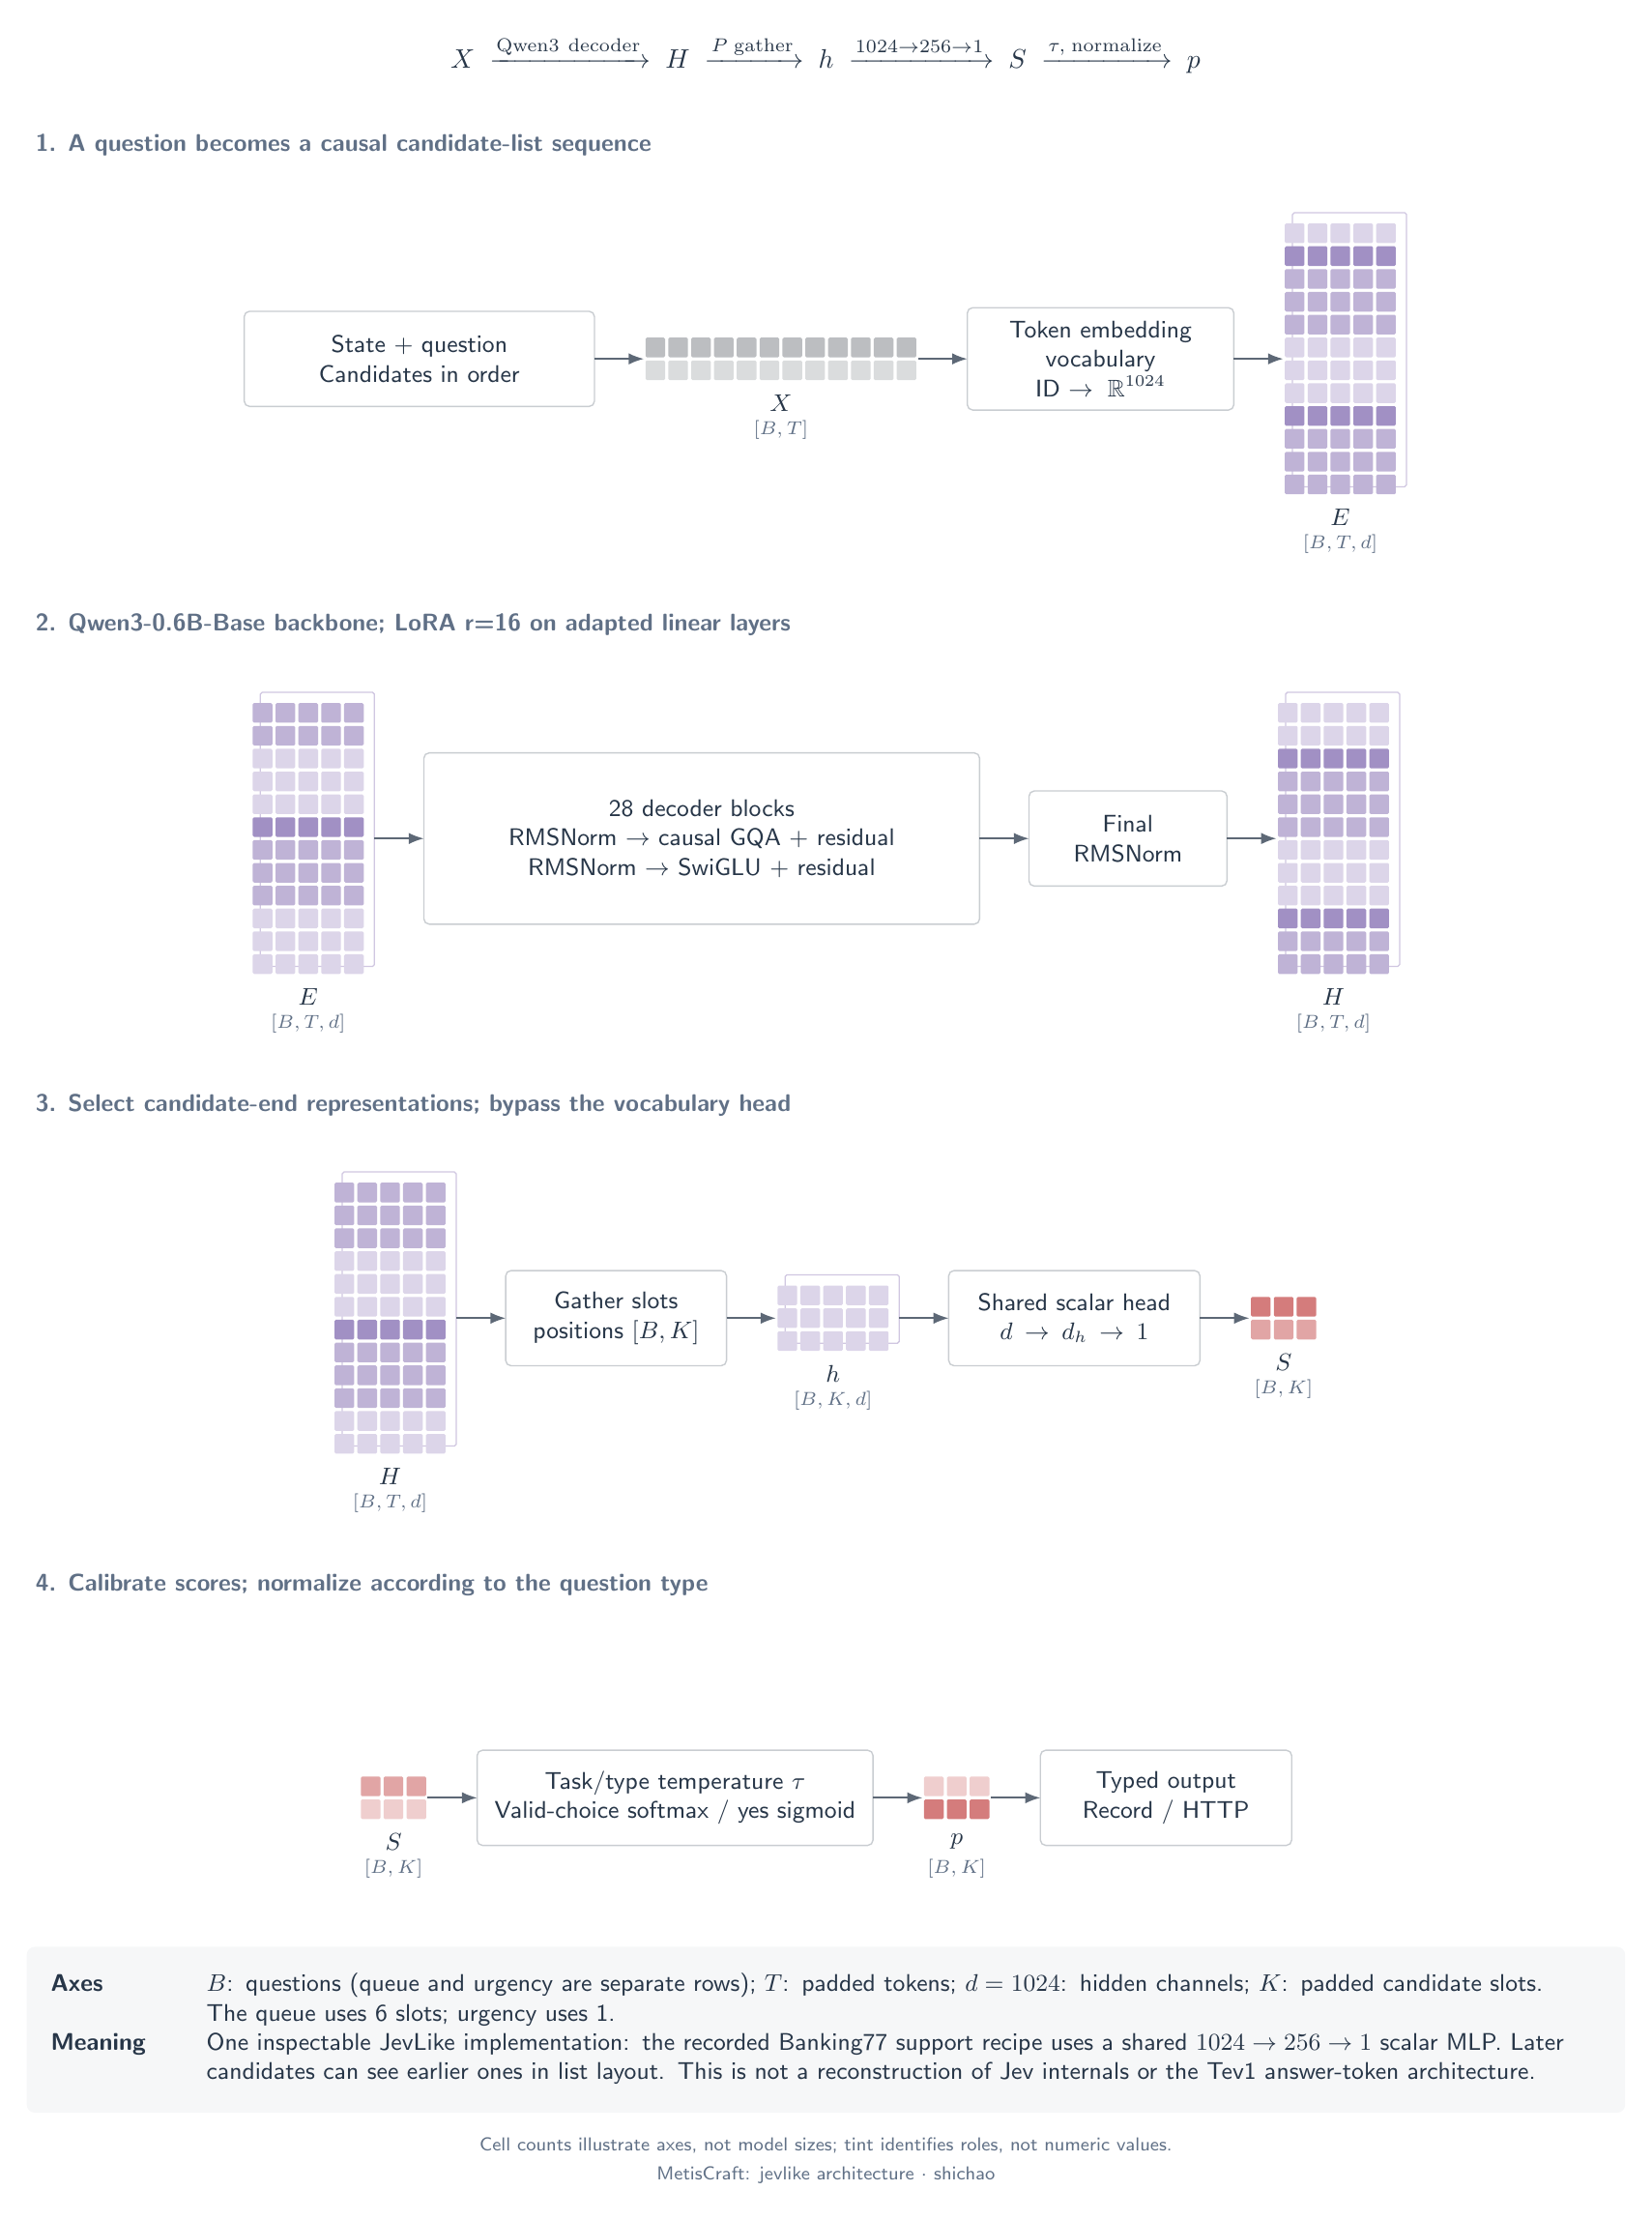
\begin{tikzpicture}[x=1cm,y=1cm,text=Ink]
\node[font=\normalsize,align=center] at (10.500,4.0) {$\displaystyle X\;\xrightarrow{\mathrm{Qwen3\ decoder}}\;H\;\xrightarrow{P\;\mathrm{gather}}\;h\;\xrightarrow{1024\to256\to1}\;S\;\xrightarrow{\tau,\;\mathrm{normalize}}\;p$};
\node[stage] at (0,2.800) {1. A question becomes a causal candidate-list sequence};
\node[operation,minimum width=4.600cm,minimum height=1.250cm,text width=4.250cm] (r0n0) at (5.165,-0.000) {State + question\\Candidates in order};
\coordinate (r0n0-w) at (2.865,-0.000);\coordinate (r0n0-e) at (7.465,-0.000);
\renewcommand{\BinarySupport}{0}
\Tensor{r0n1}{9.915}{-0.000}{2}{12}{Ctx}{0}{X}{[B,T]}
\draw[flow] (r0n0-e) -- (r0n1-w);
\node[operation,minimum width=3.500cm,minimum height=1.250cm,text width=3.150cm] (r0n2) at (14.115,-0.000) {Token embedding\\vocabulary ID $\to\mathbb{R}^{1024}$};
\coordinate (r0n2-w) at (12.365,-0.000);\coordinate (r0n2-e) at (15.865,-0.000);
\draw[flow] (r0n1-e) -- (r0n2-w);
\renewcommand{\BinarySupport}{0}
\Tensor{r0n3}{17.265}{-0.000}{12}{5}{Hid}{1}{E}{[B,T,d]}
\draw[flow] (r0n2-e) -- (r0n3-w);
\node[stage] at (0,-3.500) {2. Qwen3-0.6B-Base backbone; LoRA r=16 on adapted linear layers};
\renewcommand{\BinarySupport}{0}
\Tensor{r1n0}{3.705}{-6.300}{12}{5}{Hid}{1}{E}{[B,T,d]}
\node[operation,minimum width=7.300cm,minimum height=2.250cm,text width=6.950cm] (r1n1) at (8.875,-6.300) {28 decoder blocks\\RMSNorm $\to$ causal GQA $+$ residual\\RMSNorm $\to$ SwiGLU $+$ residual};
\coordinate (r1n1-w) at (5.225,-6.300);\coordinate (r1n1-e) at (12.525,-6.300);
\draw[flow] (r1n0-e) -- (r1n1-w);
\node[operation,minimum width=2.600cm,minimum height=1.250cm,text width=2.250cm] (r1n2) at (14.475,-6.300) {Final\\RMSNorm};
\coordinate (r1n2-w) at (13.175,-6.300);\coordinate (r1n2-e) at (15.775,-6.300);
\draw[flow] (r1n1-e) -- (r1n2-w);
\renewcommand{\BinarySupport}{0}
\Tensor{r1n3}{17.175}{-6.300}{12}{5}{Hid}{1}{H}{[B,T,d]}
\draw[flow] (r1n2-e) -- (r1n3-w);
\node[stage] at (0,-9.800) {3. Select candidate-end representations; bypass the vocabulary head};
\renewcommand{\BinarySupport}{0}
\Tensor{r2n0}{4.780}{-12.600}{12}{5}{Hid}{1}{H}{[B,T,d]}
\node[operation,minimum width=2.900cm,minimum height=1.250cm,text width=2.550cm] (r2n1) at (7.750,-12.600) {Gather slots\\positions $[B,K]$};
\coordinate (r2n1-w) at (6.300,-12.600);\coordinate (r2n1-e) at (9.200,-12.600);
\draw[flow] (r2n0-e) -- (r2n1-w);
\renewcommand{\BinarySupport}{0}
\Tensor{r2n2}{10.600}{-12.600}{3}{5}{Hid}{1}{h}{[B,K,d]}
\draw[flow] (r2n1-e) -- (r2n2-w);
\node[operation,minimum width=3.300cm,minimum height=1.250cm,text width=2.950cm] (r2n3) at (13.770,-12.600) {Shared scalar head\\$d\to d_h\to1$};
\coordinate (r2n3-w) at (12.120,-12.600);\coordinate (r2n3-e) at (15.420,-12.600);
\draw[flow] (r2n2-e) -- (r2n3-w);
\renewcommand{\BinarySupport}{0}
\Tensor{r2n4}{16.520}{-12.600}{2}{3}{Lgt}{0}{S}{[B,K]}
\draw[flow] (r2n3-e) -- (r2n4-w);
\node[stage] at (0,-16.100) {4. Calibrate scores; normalize according to the question type};
\renewcommand{\BinarySupport}{0}
\Tensor{r3n0}{4.825}{-18.900}{2}{3}{Lgt}{0}{S}{[B,K]}
\node[operation,minimum width=5.200cm,minimum height=1.250cm,text width=4.850cm] (r3n1) at (8.525,-18.900) {Task/type temperature $\tau$\\Valid-choice softmax / yes sigmoid};
\coordinate (r3n1-w) at (5.925,-18.900);\coordinate (r3n1-e) at (11.125,-18.900);
\draw[flow] (r3n0-e) -- (r3n1-w);
\renewcommand{\BinarySupport}{0}
\Tensor{r3n2}{12.225}{-18.900}{2}{3}{Lgt}{0}{p}{[B,K]}
\draw[flow] (r3n1-e) -- (r3n2-w);
\node[operation,minimum width=3.300cm,minimum height=1.250cm,text width=2.950cm] (r3n3) at (14.975,-18.900) {Typed output\\Record / HTTP};
\coordinate (r3n3-w) at (13.325,-18.900);\coordinate (r3n3-e) at (16.625,-18.900);
\draw[flow] (r3n2-e) -- (r3n3-w);
\Meaning{0}{-20.850}{21.000}{Axes}{$B$: questions (queue and urgency are separate rows); $T$: padded tokens; $d=1024$: hidden channels; $K$: padded candidate slots. The queue uses 6 slots; urgency uses 1.}{Meaning}{One inspectable JevLike implementation: the recorded Banking77 support recipe uses a shared $1024\to256\to1$ scalar MLP. Later candidates can see earlier ones in list layout. This is not a reconstruction of Jev internals or the Tev1 answer-token architecture.}
\node[font=\scriptsize,text=Muted,anchor=north,align=center] at ($(meaning.south)+(0,-.2)$) {Cell counts illustrate axes, not model sizes; tint identifies roles, not numeric values.\\[3pt]MetisCraft: jevlike architecture $\cdot$ shichao};
\end{tikzpicture}
\end{document}
